\chapter{Neuronavegação}
\label{sec:neuronavegador}

A introdução sobre a neuronavegação é feita na seção~\ref{sec:neuronavegador_intro}, é recomendável a leitura caso não tenha sido feita.

Para utilizar o neuronavegador, é necessário habilitar o modo de neuronavegação do InVesalius selecionando no menu \textbf{Modo} em seguida \textbf{Navegação} (figura~\ref{fig:nav_menu_pt}). Será ativada uma nova aba "Sistema de navegação" que ficará visível no painel à esquerda da janela principal como é apresentado na figura~\ref{fig:nav_painel_pt}.

\begin{figure}[!htb]
\centering
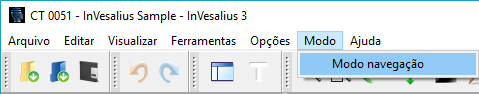
\includegraphics[scale=0.4]{nav_menu_pt.png}
\caption{Menu para ativar o modulo de neuronavegação.}
\label{fig:nav_menu_pt}
\end{figure}

\begin{figure}[!htb]
\centering
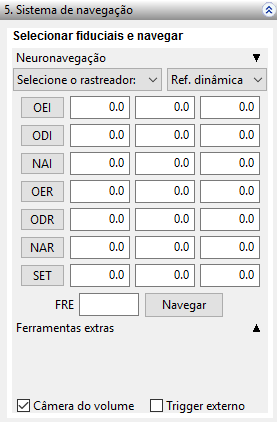
\includegraphics[scale=0.6]{nav_painel_pt.png}
\caption{Aba do sistema de neuronavegação.}
\label{fig:nav_painel_pt}
\end{figure}

\section{Rastreadores espaciais e modo de referência}

O sistema de neuronavegação se comunica com vários sistemas de rastreamento espacial. Atualmente, suporta os dispositivos fabricados pela ClaroNav (figura~\ref{fig:tracker_claron}) e Polhemus (figura~\ref{fig:tracker_polhemus}). 

O usuário deve selecionar o dispositivo correspondente no botão \textbf{Selecione o rastreador:}, figura~\ref{fig:nav_select_tracker}.  Caso o usuário não possua nenhum dos rastreadores suportados e deseja realizar um teste do sistema, deve selecionar a opção \textbf{Depurar rastreador} e realizar normalmente os procedimentos que serão citados a seguir. Nessa opção, trata-se de uma simulação, do qual serão geradas coordenadas aleatórias.

\begin{figure}[!htb]
\centering
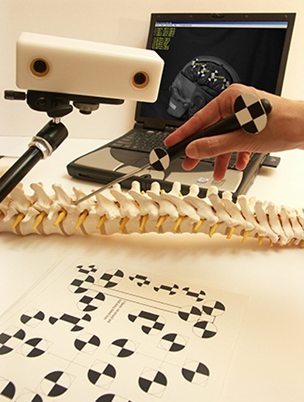
\includegraphics[scale=0.4]{tracker_claron.png}
\caption{Rastreador Claron - www.claronav.com/microntracker/.}
\label{fig:tracker_claron}
\end{figure}

\begin{figure}[!htb]
\centering
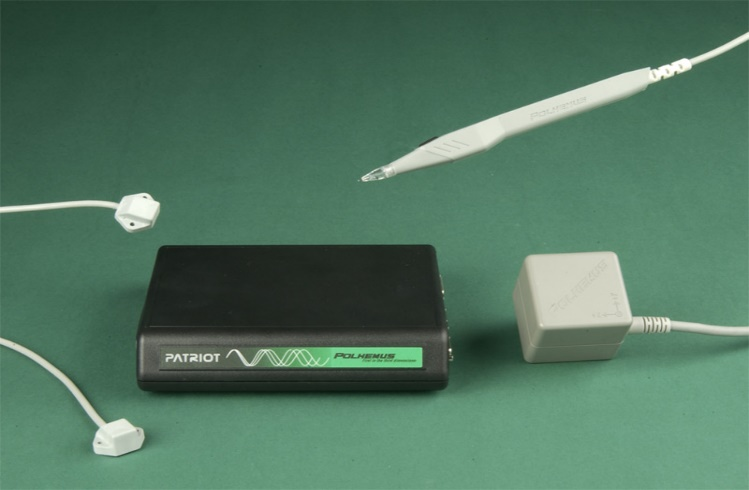
\includegraphics[scale=0.5]{tracker_polhemus.jpg}
\caption{Rastreador Polhemus - http://polhemus.com/motion-tracking/overview/.}
\label{fig:tracker_polhemus}
\end{figure}

\begin{figure}[!htb]
\centering
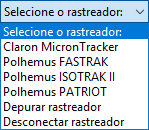
\includegraphics[scale=0.5]{nav_select_tracker_pt.png}
\caption{Menu para seleção de rastreador.}
\label{fig:nav_select_tracker}
\end{figure}

É possível realizar a navegação com dois diferentes tipos de referência, estático e dinâmico (figura~\ref{fig:nav_menu_ref}). No modo estático as coordenadas do dispositivo de rastreamento são detectadas com apenas uma sonda. Este modo de navegação é chamado de modo de referência estática porque a cabeça dos sujeitos deve permanecer estática na posição em que foram detectados os pontos fiduciais (Mais informações na seção~\ref{sec:corregistro}). 
Para evitar problemas relacionados com o movimento da cabeça, alguns dispositivos de rastreamento fornecem uma sonda de referência. A sonda de referência pode ser ligada a uma parte não móvel da cabeça, por exemplo testa, para acompanhar as translações e rotações durante o procedimento de navegação. O uso de uma sonda de referência é o chamado modo de referência dinâmica.

\begin{figure}[!htb]
\centering
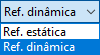
\includegraphics[scale=0.5]{nav_menu_ref.png}
\caption{Menu para seleção de referência.}
\label{fig:nav_menu_ref}
\end{figure}

\section{Corregistro}
\label{sec:corregistro}

O objetivo do corregistro é estabelecer uma relação entre o espaço de coordenadas do rastreador espacial e o espaço de coordenadas virtual (imagem). Para realizar o corregistro, o usuário deve selecionar três marcadores fiduciais na imagem, para isso primeiramente deverá ativar o recurso de \textbf{Correspondência entre as orientações axial, sagital e coronal} (ver seção~\ref{sec:corresp_all_orient}), coletar as três coordenadas fiduciais usando a sonda do dispositivo de rastreamento. Os fiduciais mais utilizados são o trago auricular esquerdo, trago auricular direito e a fossa nasal. A figura~\ref{fig:nav_selec_coord} ilustra a coleta dos pontos fiduciais. Quando é selecionado algum ponto fiducial na imagem, automaticamente é criado um marcador (esfera da cor verde) no volume, figura~\ref{fig:nav_balls_in_head}.

\begin{figure}[!htb]
\centering
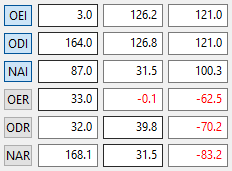
\includegraphics[scale=0.5]{nav_selec_coord_pt.png}
\caption{Botões e coordenadas para seleção de pontos fiduciais.}
\label{fig:nav_selec_coord}
\end{figure}

As siglas dos botões para coleta dos fiduciais representam:

\begin{itemize}
	\item OEI: trago auricular esquerdo na imagem
	\item ODI: trago auricular direito na imagem
	\item NAI: fossa nasal na imagem
	\item OER: trago auricular esquerdo no rastreador
	\item OER: trago auricular direito no rastreador
	\item NAR: fossa nasal esquerdo no rastreador
\end{itemize}

\begin{figure}[!htb]
\centering
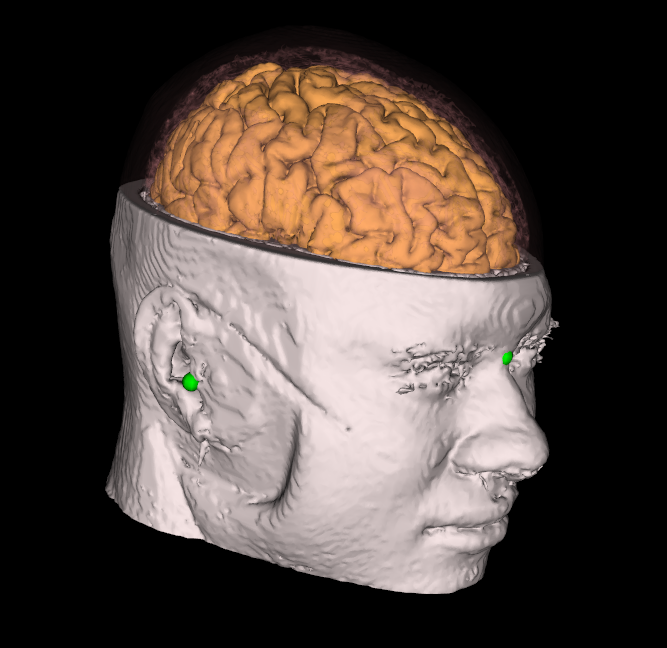
\includegraphics[scale=0.5]{nav_balls_in_head.png}
\caption{Criação de marcadores nos pontos fiduciais da imagem.}
\label{fig:nav_balls_in_head}
\end{figure}


\section{Erro de registro fiducial e navegação}

Após o usuário selecionar os três pontos fiduciais na imagem e os respectivos pontos com o rastreador espacial, o próximo passo é clicar no \textbf{botão Navegar} e o procedimento de navegação será iniciado. Para pausar a navegação, basta clicar novamente no \textbf{botão Navegar}. Automaticamente após selecionado a navegação é calculado o erro de registro fiducial, conhecido como \textit{Fiducial Registration Error} (FRE). Esse erro representa a distância média quadrática do ponto fiducial na imagem com o respectivo ponto fiducial obtido após realizado o corregistro. 

Ao lado do botão de navegação, há a caixa de texto respectivo ao FRE. Se o FRE apresentar um valor alto (acima de 3 mm) a navegação não será precisa e a caixa de texto ficará vermelha, figura~\ref{fig:nav_fre_error}, recomenda-se que o corregistro seja refeito. Caso contrário, para FRE menor que 3 mm a caixa de texto fica verde, representando que a navegação terá precisão aceitável, figura~\ref{fig:nav_fre_ok}.

\begin{figure}[!htb]
\centering
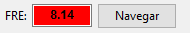
\includegraphics[scale=0.6]{nav_fre_error_pt.png}
\caption{Botão de navegação e FRE com valor elevado para navegação.}
\label{fig:nav_fre_error}
\end{figure}

\begin{figure}[!htb]
\centering
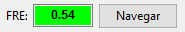
\includegraphics[scale=0.6]{nav_fre_ok_pt.png}
\caption{Botão de navegação e FRE com valor aceitável para navegação.}
\label{fig:nav_fre_ok}
\end{figure}

\section{Marcadores}

Durante a navegação, é possível criar marcadores esféricos no volume 3D. Para acessar essa função, basta clicar na aba \textbf{Ferramentas extras}, figura~\ref{fig:nav_extra_tools}.

\begin{figure}[!htb]
\centering
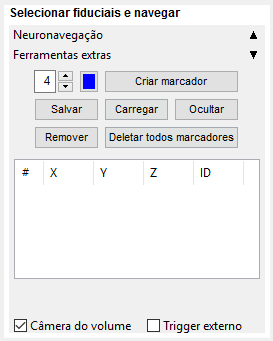
\includegraphics[scale=0.6]{nav_extra_tools_pt.png}
\caption{Aba para manipulação de marcadores.}
\label{fig:nav_extra_tools}
\end{figure}

A criação de marcadores pode ser executada clicando no botão correspondente, com isso será criado um marcador na posição da cruz vermelha com as características escolhidas na aba, figura~\ref{fig:nav_extra_tools}. O número 4 representa o tamanho do raio da esfera que será criada. Ao lado do tamanho do marcador é possível definir a cor da esfera (figura~\ref{fig:nav_vol_with_markers}). 

Caso o usuário desejar identificar o marcador criado no volume, um \textbf{clique duplo com o botão esquerdo do mouse} deve ser realizado no marcador desejado, com isso o respectivo começará a piscar.

É possível criar uma identificação para o marcador, para isso, deve-se clicar com o botão direto sobre o marcador desejado e selecionar \textbf{Editar ID}, figura~\ref{fig:nav_id_list_markers}, será aberto uma janela para o usuário digitar a identificação, figura~\ref{fig:nav_edit_id_markers}.

\begin{figure}[!htb]
\centering
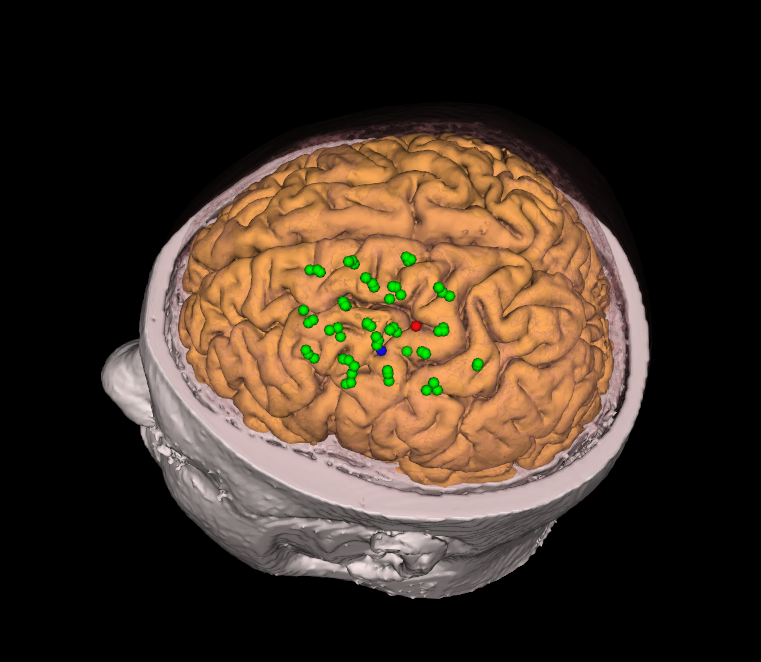
\includegraphics[scale=0.4]{nav_vol_with_markers.png}
\caption{Volume com marcadores em diferentes cores.}
\label{fig:nav_vol_with_markers}
\end{figure} 

\begin{figure}[!htb]
\centering
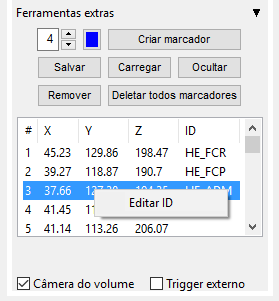
\includegraphics[scale=0.6]{nav_id_list_markers_pt.png}
\caption{Aba para manipulação de marcadores.}
\label{fig:nav_id_list_markers}
\end{figure} 

\begin{figure}[!htb]
\centering
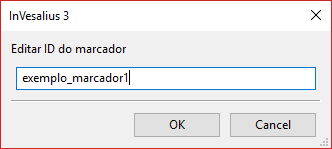
\includegraphics[scale=0.6]{nav_edit_id_markers_pt.png}
\caption{Janela para editar identificação do marcador.}
\label{fig:nav_edit_id_markers}
\end{figure} 

A exportação dos marcadores é feita através do \textbf{botão salvar}, a extensão do arquivo gerado é o .mks. Essa extensão de arquivo pode ser aberta por processadores de texto como bloco de notas. O arquivo possui as coordenadas $X$, $Y$ e $Z$ seguido o código $RGB$, tamanho de marcador e a identificação. Posteriormente, esse arquivo pode ser importado através do \textbf{botão Carregar}.

Caso o usuário desejar excluir apenas um marcador basta \textbf{selecionar} o item desejado na lista e clicar no \textbf{botão Remover}, também existe a opção de excluir todos os marcadores criados, \textbf{Deletar todos marcadores}. Além disso, pode-se ocultar/mostrar a exibição dos marcadores no volume pelo \textbf{botão ocultar/mostrar}.

\section{Caixas de seleção, trigger externo}

Outra maneira para criação de marcadores é a monitoração externa de trigger. Para ativa-la basta selecionar a caixa de seleção \textbf{Trigger externo}. Essa função foi desenvolvida para comunicar dispositivos EMT e criar automaticamente o marcador em posições onde os pulsos foram aplicados. No entanto, outras aplicações são possíveis de acordo com a necessidade do usuário.
A comunicação com o dispositivo externo é feita através da porta serial COM1, e basta enviar qualquer sinal do tipo RS-232 em uma velocidade \textit{baud rate} de 9600 no pino de recepção que será criado um marcador na atual posição da cruz.

\section{Câmera do volume}

O posicionamento da câmera do volume é atualizado automaticamente, tanto pela posição da cruz vermelha das fatias quanto pela posição da sonda durante a navegação. O usuário pode desabilitar a atualização automática e atualizar a câmera manualmente. O posicionamento será alterado caso o usuário o fizer na janela de volume.  Para isso, basta desmarcar a caixa de seleção \textbf{Câmera do volume}.
